% **************************************************************************************************************
% A Classic Thesis Style
% An Homage to The Elements of Typographic Style
%
% Copyright (C) 2012 Andr\'e Miede http://www.miede.de
%
% If you like the style then I would appreciate a postcard. My address 
% can be found in the file ClassicThesis.pdf. A collection of the 
% postcards I received so far is available online at 
% http://postcards.miede.de
%
% License:
% This program is free software; you can redistribute it and/or modify
% it under the terms of the GNU General Public License as published by
% the Free Software Foundation; either version 2 of the License, or
% (at your option) any later version.
%
% This program is distributed in the hope that it will be useful,
% but WITHOUT ANY WARRANTY; without even the implied warranty of
% MERCHANTABILITY or FITNESS FOR A PARTICULAR PURPOSE.  See the
% GNU General Public License for more details.
%
% You should have received a copy of the GNU General Public License
% along with this program; see the file COPYING.  If not, write to
% the Free Software Foundation, Inc., 59 Temple Place - Suite 330,
% Boston, MA 02111-1307, USA.
%
% **************************************************************************************************************
% Note:
%    * You must not use "u etc. in strings/commands that will be spaced out (use \"u or real umlauts instead)
%    * New enumeration (small caps): \begin{aenumerate} \end{aenumerate}
%    * For margin notes: \marginpar or \graffito{}
%    * Do not use bold fonts in this style, it is designed around them
%    * Use tables as in the examples
%    * See classicthesis-preamble.sty for useful commands
% **************************************************************************************************************
% To Do:
%		 * [high] Check this out: http://www.golatex.de/koma-script-warnung-in-verbindung-mit-listings-package-t2058.html
%    * [medium] mathbb in section-titles/chapter-titles => disappears somehow in headlines!!!
% **************************************************************************************************************
\documentclass[ twoside,openright,titlepage,numbers=noenddot,headinclude,%1headlines,% letterpaper a4paper
                footinclude=true,cleardoublepage=empty,abstractoff, % <--- obsolete, remove (todo)
                BCOR=5mm,paper=a4,fontsize=11pt,%11pt,a4paper,%
                UKenglish,%
                ]{scrreprt}

%********************************************************************
% Note: Make all your adjustments in here
%*******************************************************

% ****************************************************************************
% 1. Configure classicthesis for your needs here, e.g., remove "drafting" below 
% in order to deactivate the time-stamp on the pages
% ****************************************************************************
\PassOptionsToPackage{
  eulerchapternumbers,
  dottedtoc,
  listings,
  % drafting,
  pdfspacing,
  %floatperchapter,
  linedheaders,
  subfig,
  beramono,
  eulermath,
  parts
}{classicthesis}

% ********************************************************************
% Triggers for this config
% ******************************************************************** 
\usepackage{ifthen}
\newboolean{enable-backrefs} % enable backrefs in the bibliography
\setboolean{enable-backrefs}{false} % true false
% ****************************************************************************

% ****************************************************************************
% 2. Personal data and user ad-hoc commands
% ****************************************************************************

\newcommand{\myTitle}{Retext\xspace}
\newcommand{\mySubtitle}{Design of an extensible system for analysing and manipulating natural language\xspace}
\newcommand{\myDegree}{\xspace}
\newcommand{\myName}{Titus E. C. Wormer\xspace}
\newcommand{\myProf}{\xspace}
\newcommand{\myOtherProf}{\xspace}
\newcommand{\mySupervisor}{Justus Sturkenboom\xspace}
\newcommand{\myFaculty}{Communication and Multimedia Design\xspace}
\newcommand{\myDepartment}{School of Design and Communication\xspace}
\newcommand{\myUni}{Amsterdam University of Applied Sciences\xspace}
\newcommand{\myLocation}{Delft\xspace}
\newcommand{\myTime}{August 2014\xspace}
\newcommand{\myVersion}{version 0.3\xspace}

% ********************************************************************
% Setup, finetuning, and useful commands
% ********************************************************************
\newcounter{dummy} % necessary for correct hyperlinks (to index, bib, etc.)
\newlength{\abcd} % for ab..z string length calculation
\providecommand{\mLyX}{L\kern-.1667em\lower.25em\hbox{Y}\kern-.125emX\@}
\newcommand{\ie}{i.\,e.}
\newcommand{\Ie}{I.\,e.}
\newcommand{\eg}{e.\,g.}
\newcommand{\Eg}{E.\,g.} 
% ****************************************************************************


% ****************************************************************************
% 3. Loading some handy packages
% ****************************************************************************
% ******************************************************************** 
% Packages with options that might require adjustments
% ******************************************************************** 
\PassOptionsToPackage{utf8}{inputenc}
\usepackage{inputenc}

\PassOptionsToPackage{british}{babel}
\usepackage[]{babel}

% math environments and more by the AMS 
% \PassOptionsToPackage{fleqn}{amsmath}
% \usepackage{amsmath}

% ******************************************************************** 
% General useful packages
% ******************************************************************** 
\PassOptionsToPackage{T1}{fontenc} % T2A for cyrillics
\usepackage{fontenc}

% fix warning with missing font shapes
\usepackage{textcomp}

% fix warnings when using KOMA with listings package
\usepackage{scrhack}

% to get the spacing after macros right
\usepackage{xspace}

% get marginpar right
\usepackage{mparhack}

% fixes some LaTeX stuff 
\usepackage{fixltx2e}

\PassOptionsToPackage{printonlyused,smaller}{acronym}

% nice macros for handling all acronyms in the thesis
\usepackage{acronym}

% for MinionPro
%\renewcommand*{\acsfont}[1]{\textssc{#1}}

% fix the list of acronyms
\renewcommand{\bflabel}[1]{{#1}\hfill}
% ****************************************************************************


% ****************************************************************************
% 4. Setup floats: tables, (sub)figures, and captions
% ****************************************************************************
\usepackage{tabularx} % better tables
% increase table row height
\setlength{\extrarowheight}{3pt}

\newcommand{\tableheadline}[1]{\multicolumn{1}{c}{\spacedlowsmallcaps{#1}}}

% to be used with each float for alignment
\newcommand{\myfloatalign}{\centering}
\usepackage{caption}
\captionsetup{format=hang,font=small}
\usepackage{subfig}  

% ****************************************************************************


% ****************************************************************************
% 5. Setup code listings
% ****************************************************************************
\usepackage{listings} 
%\lstset{emph={trueIndex,root},emphstyle=\color{BlueViolet}}%\underbar} % for special keywords

% \usepackage{color}

\lstset{language=[LaTeX]Tex,IDL%C++,
    basicstyle=\ttfamily,
    sensitive=true,
    breaklines=true,
    tabsize=2
    numbers=none,%left,%
    numberstyle=\scriptsize,%\tiny
    stepnumber=5,
    numbersep=8pt,
    showstringspaces=false,
    frameround=ftff,
    frame=single,
    belowcaptionskip=.75\baselineskip
    %frame=L
} 
% ****************************************************************************

% ****************************************************************************
% 6. PDFLaTeX, hyperreferences and citation backreferences
% ****************************************************************************
% ********************************************************************
% Using PDFLaTeX
% ********************************************************************
\PassOptionsToPackage{
  pdftex,
  hyperfootnotes=false,
  pdfpagelabels
}{hyperref}
\usepackage{hyperref}  % backref linktocpage pagebackref

\pdfcompresslevel=9
\pdfadjustspacing=1 
\PassOptionsToPackage{pdftex}{graphicx}
	\usepackage{graphicx} 

% ********************************************************************
% Setup the style of the backrefs from the bibliography
% (translate the options to any language you use)
% ********************************************************************
\newcommand{\backrefnotcitedstring}{\relax}%(Not cited.)
\newcommand{\backrefcitedsinglestring}[1]{(Cited on page~#1.)}
\newcommand{\backrefcitedmultistring}[1]{(Cited on pages~#1.)}
\ifthenelse{\boolean{enable-backrefs}}%
{%
		\PassOptionsToPackage{hyperpageref}{backref}
		\usepackage{backref} % to be loaded after hyperref package 
		   \renewcommand{\backreftwosep}{ and~} % separate 2 pages
		   \renewcommand{\backreflastsep}{, and~} % separate last of longer list
		   \renewcommand*{\backref}[1]{}  % disable standard
		   \renewcommand*{\backrefalt}[4]{% detailed backref
		      \ifcase #1 %
		         \backrefnotcitedstring%
		      \or%
		         \backrefcitedsinglestring{#2}%
		      \else%
		         \backrefcitedmultistring{#2}%
		      \fi}%
}{\relax}    

% ********************************************************************
% Hyperreferences
% ********************************************************************
\hypersetup{%
    %draft,	% = no hyperlinking at all (useful in b/w printouts)
    colorlinks=false,
    linktocpage=true,
    pdfstartpage=3,
    pdfstartview=FitV,

    % linktocpage=false,
    % pdfborder={0 0 0},
    % pdfstartpage=3,
    % pdfstartview=FitV,
    breaklinks=true,
    pdfpagemode=UseNone,
    pageanchor=true,
    pdfpagemode=UseOutlines,
    plainpages=false,
    bookmarksnumbered,
    bookmarksopen=true,
    bookmarksopenlevel=1,
    hypertexnames=true,
    pdfhighlight=/O,
    % nesting=true,
    % frenchlinks,
    urlcolor=webbrown,
    linkcolor=RoyalBlue,
    citecolor=webgreen,
    % pagecolor=RoyalBlue,%
    % urlcolor=Black,
    % linkcolor=Black,
    % citecolor=Black,
    %pagecolor=Black,
    pdftitle={\myTitle},
    pdfauthor={\textcopyright\ \myName, \myUni, \myFaculty},
    pdfsubject={\mySubtitle},
    pdfkeywords={},
    pdfcreator={pdfLaTeX},
    pdfproducer={LaTeX with hyperref and classicthesis}
}   

% ********************************************************************
% Setup autoreferences
% ********************************************************************
% There are some issues regarding autorefnames
% http://www.ureader.de/msg/136221647.aspx
% http://www.tex.ac.uk/cgi-bin/texfaq2html?label=latexwords
% you have to redefine the makros for the 
% language you use, e.g., american, ngerman
% (as chosen when loading babel/AtBeginDocument)
% ********************************************************************
\makeatletter
\@ifpackageloaded{babel}%
    {%
       \addto\extrasamerican{%
					\renewcommand*{\figureautorefname}{Figure}%
					\renewcommand*{\tableautorefname}{Table}%
					\renewcommand*{\partautorefname}{Part}%
					\renewcommand*{\chapterautorefname}{Chapter}%
					\renewcommand*{\sectionautorefname}{Section}%
					\renewcommand*{\subsectionautorefname}{Section}%
					\renewcommand*{\subsubsectionautorefname}{Section}% 	
				}%
       \addto\extrasngerman{% 
					\renewcommand*{\paragraphautorefname}{Absatz}%
					\renewcommand*{\subparagraphautorefname}{Unterabsatz}%
					\renewcommand*{\footnoteautorefname}{Fu\"snote}%
					\renewcommand*{\FancyVerbLineautorefname}{Zeile}%
					\renewcommand*{\theoremautorefname}{Theorem}%
					\renewcommand*{\appendixautorefname}{Anhang}%
					\renewcommand*{\equationautorefname}{Gleichung}%        
					\renewcommand*{\itemautorefname}{Punkt}%
				}%	
			% Fix to getting autorefs for subfigures right (thanks to Belinda Vogt for changing the definition)
			\providecommand{\subfigureautorefname}{\figureautorefname}%  			
    }{\relax}
\makeatother


% ****************************************************************************
% 7. Last calls before the bar closes
% ****************************************************************************
% ********************************************************************
% Development Stuff
% ********************************************************************
% \listfiles
% \PassOptionsToPackage{l2tabu,orthodox,abort}{nag}
% \usepackage{nag}
% \PassOptionsToPackage{warning, all}{onlyamsmath}
% \usepackage{onlyamsmath}

% ********************************************************************
% Last, but not least...
% ********************************************************************
\usepackage{classicthesis} 
% ****************************************************************************

% ****************************************************************************
% 8. Further adjustments (experimental)
% ****************************************************************************
% ********************************************************************
% Changing the text area
% ********************************************************************
\linespread{1.05} % a bit more for Palatino
\areaset[current]{312pt}{761pt} % 686 (factor 2.2) + 33 head + 42 head \the\footskip
\setlength{\marginparwidth}{7em}
\setlength{\marginparsep}{2em}

% ********************************************************************
% Using different fonts
% ********************************************************************
\usepackage[oldstylenums]{kpfonts} % oldstyle notextcomp
\usepackage[osf]{libertine}
% \usepackage{hfoldsty} % Computer Modern with osf
% \usepackage[light,condensed,math]{iwona}
% \renewcommand{\sfdefault}{iwona}
% \usepackage{lmodern} % <-- no osf support :-(
% \usepackage[urw-garamond]{mathdesign} % <-- no osf support :-(
% ****************************************************************************


%********************************************************************
% CUSTOM!
%*******************************************************
\usepackage[utf8]{inputenx}

\usepackage[xindy,acronym,nomain]{glossaries}
\glsdisablehyper % Disable links from items to glossary.
\makeglossaries

%*******************************************************
% Glossary list
%*******************************************************

\newacronym{nlp}{nlp}{Natural Language Processing}
\newacronym{ibm}{ibm}{International Business Machines Corporation}
\newacronym{pos}{pos}{Part-of-Speech}
\newacronym{api}{api}{Application Programming Interface}
\newacronym{http}{http}{Hypertext Transfer Protocol}
\newacronym{html}{html}{Hypertext Markup Language}
\newacronym{html5}{html5}{Hypertext Markup Language 5}
\newacronym{ajax}{ajax}{Asynchronous JavaScript and XML}
\newacronym{nlcst}{nlcst}{Natural Language Concrete Syntax Tree}
\newacronym{textom}{TextOM}{Text Object Model}
\newacronym{css}{css}{Cascading Style Sheets}
\newacronym{ast}{ast}{Abstract Syntax Tree}
\newacronym{cst}{cst}{Concrete Syntax Tree}
\newacronym{dom}{dom}{Document Object Model}
\newacronym{php}{php}{PHP: Hypertext Preprocessor}
\newacronym{mongodb}{mongodb}{Mongo Database}
\newacronym{mysql}{mysql}{My Structured Query Language}
\newacronym{mit}{mit}{Michigan Institute of Technology}
\newacronym{jscs}{jscs}{JavaScript Code Style Checker}
\newacronym{jsdoc}{jsdoc}{JavaScript Documentation}
\newacronym{ci}{ci}{Continuous Integration}
\newacronym{cmd}{cmd}{Communication and Muldimedia Design}

\newglossaryentry{npm}
{
  name=npm,
  description={Package manager for, and included in, Node.js}
}

\newglossaryentry{ecmascript}
{
  name=ECMAScript,
  description={More commonly known as JavaScript, ECMAScript is a language widely used for client-side programming on the web}
}


%********************************************************************
% Hyphenation
%*******************************************************
%\hyphenation{put special hyphenation here}

% ********************************************************************
% GO!GO!GO! MOVE IT!
%*******************************************************
\begin{document}
\frenchspacing
\raggedbottom
\selectlanguage{UKenglish} % american
%\renewcommand*{\bibname}{new name}
%\setbibpreamble{}
\pagenumbering{roman}
\pagestyle{plain}
%********************************************************************
% Frontmatter
%*******************************************************
%*******************************************************
% Cover
%*******************************************************
\thispagestyle{empty}
\begin{addmargin}[-1cm]{-3cm}
  \begin{center}

  \spacedlowsmallcaps{\myName} \\ \medskip

  \begingroup
    \color{Maroon}\spacedallcaps{\myTitle}
  \endgroup

  \end{center}
\end{addmargin}

%*******************************************************
% Titlepage
%*******************************************************
\begin{titlepage}
	% if you want the titlepage to be centered, uncomment and fine-tune the line below (KOMA classes environment)
	\begin{addmargin}[-1cm]{-3cm}
    \begin{center}
        \large  

        \hfill

        \vfill

        \begingroup
            \color{Maroon}\spacedallcaps{\myTitle} \\ \bigskip
        \endgroup

        \spacedlowsmallcaps{\myName}

        \vfill

        \mySubtitle \\ \medskip   
        %\myDegree \\
        %\myDepartment \\                            
        %\myFaculty \\
        %\myUni \\ \bigskip

        \myTime\ -- \myVersion

        \vfill                      

    \end{center}  
  \end{addmargin}       
\end{titlepage}   
\thispagestyle{empty}

\hfill

\vfill

\noindent\myName: \textit{\myTitle,} \mySubtitle, %\myDegree, 
\textcopyright\ \myTime

%\bigskip
%
%\noindent\spacedlowsmallcaps{Supervisors}: \\
%\myProf \\
%\myOtherProf \\ 
%\mySupervisor
%
%\medskip
%
%\noindent\spacedlowsmallcaps{Location}: \\
%\myLocation
%
%\medskip
%
%\noindent\spacedlowsmallcaps{Time Frame}: \\
%\myTime

\cleardoublepage%*******************************************************
% Acknowledgments
%*******************************************************
\pdfbookmark[1]{Acknowledgments}{acknowledgments}

\begingroup
\let\clearpage\relax
\let\cleardoublepage\relax
\let\cleardoublepage\relax
\chapter*{Acknowledgments}

Thanks to my supervisor Justus for the trust in me and my work, and for
allowing me to produce a product and thesis that perhaps not every CMD
professional understands, but most certainly falls within our field.

\endgroup

\cleardoublepage%*******************************************************
% Dedication
%*******************************************************
\thispagestyle{empty}
\refstepcounter{dummy}
\pdfbookmark[1]{Dedication}{Dedication}

\input{2.dedication.tex}

\cleardoublepage%*******************************************************
% Abstract
%*******************************************************
% to have the abstract a bit from the rest in the toc
\refstepcounter{dummy}
\addtocontents{toc}{\protect\vspace{\beforebibskip}}
\addcontentsline{toc}{chapter}{\tocEntry{Abstract}}

\begingroup
\let\clearpage\relax
\let\cleardoublepage\relax
\let\cleardoublepage\relax

\chapter*{Abstract}

This document captures the use cases and requirements for designing and
standardising a solution for textual manipulation and analysis in
\gls{ecmascript}. In addition, this paper presents an implementation that
meets these requirements and answers these use cases.

\endgroup


\cleardoublepage%*******************************************************
% Abstract
%*******************************************************
% to have the introduction a bit from the rest in the toc
\refstepcounter{dummy}
\addtocontents{toc}{\protect\vspace{\beforebibskip}}
\addcontentsline{toc}{chapter}{\tocEntry{Introduction}}

\begingroup
\let\clearpage\relax
\let\cleardoublepage\relax
\let\cleardoublepage\relax

\chapter*{Introduction}

\Gls{nlp}, a field of computer science, artificial intelligence, and
  linguistics concerned with the interaction between computers and human
  languages, is becoming more important in society.
For\,example, search engines provide answers before being questioned,
  intelligence agencies detect threats of violence in text messages, and
  e-mail applications know if you forgot to include an attachment.

Despite increased interest, web developers trying to solve \gls{nlp} problems
  reinvent the wheel over and over.
There are tools, especially for other platforms---such\,as in Python
  \autocite{nltk-source} and Java \autocite{opennlp-source}---but they either
  take a too na\"ive approach\footnote{Such\,as ignoring white space
    \autocite{loadfive/knwl-source-code}, implementing a na\"ive
    definition of ``words'' \autocite{nhunzaker/speakeasy-source-code},
    or by using an inadequate algorithm to detect sentences
    \autocite[][]{nytimes/emphasis-source-code}.}, or try to do
  everything\footnote{Although a do-all library
    \autocite[such\,as][]{NaturalNode/natural-source-code} works well on
    server side platforms, it fares less well on the web, where modularity
    and moderation
  are in order.}.
What is missing is a standard representation of the grammatical hierarchy
  of text and a standard for multipurpose analysis of natural language.

My initial interest in natural language was sparked by typography, when I
  felt the need to create a typographically beautiful website, somewhere in
  the summer of 2013.
I felt a craving to apply the tried-and-true practices of typography found on
  paper, to the web.
I was inspired by how these practices were available on other platforms,
  on \TeX{} or \LaTeX, with tools such\,as \emph{microtype}
  \autocite{microtype}, and the \emph{ClassicThesis} theme
  \autocite{classicthesis} based on \emph{The Elements of Typographic Style}
  \autocite{bringhurst-element-typographic-style}.

My interest for fixing typography on the web was piqued.
Thus, I began work on \emph{MicroType.js}, an unpublished library, to
  enable several graphic and typographic practices on the web.
Examples include automatic initials, ligatures, optical margin alignment,
  acronym recognition, smart punctuation, automatic hyphenation, character
  transpositions, and more.
The possibilities were vast, but I noticed how the underlying parser and data
  representation were incomplete.
How words, white space, punctuation, and sentences were defined, was not
  good enough.
The website never came into existence, but during this thesis, I could
  finally fix this problem.
While working on this thesis, the specification and the product, I developed
  a well thought out and substantiated solution.

\emph{Retext}---the implementation introduced in this thesis---and other
  projects in the \emph{Retext} family are a new approach to the syntax of
  natural text.
Together they form an extensible system for multipurpose analysis of natural
  language in \gls{ecmascript}.

To reach this goal, I have organised my paper into six\,main chapters.
In the first\,chapter the scope of this paper is defined and current
  implementations are reviewed, what they lack and where they excel.
Subsequently, the second\,chapter state a research objective and drafts
  research questions.
The third\,chapter defines conditions for such a proposal, where I touch
  upon the target audience, use cases, and requirements.
In the fourth\,chapter, a better implementation is proposed and its
  architectural design is showed.

The fifth\,chapter describes the steps taken to validate the proposal.
I conclude with a sixth\,chapter that offers information on expanding the
  proposal.

\endgroup


%\cleardoublepage\include{FrontBackmatter/Foreword}
% \cleardoublepage%*******************************************************
% Publications
%*******************************************************
\pdfbookmark[1]{Publications}{publications}
\chapter*{Publications}
Some ideas and figures have appeared previously in the following publications:

\bigskip

\noindent Put your publications from the thesis here. The packages \texttt{multibib} or \texttt{bibtopic} etc. can be used to handle multiple different bibliographies in your document.
% \cleardoublepage%*******************************************************
% Acknowledgments
%*******************************************************
\pdfbookmark[1]{Acknowledgments}{acknowledgments}

\begin{flushright}{\slshape    
    We have seen that computer programming is an art, \\ 
    because it applies accumulated knowledge to the world, \\ 
    because it requires skill and ingenuity, and especially \\
    because it produces objects of beauty.} \\ \medskip
    --- \defcitealias{knuth:1974}{Donald E. Knuth}\citetalias{knuth:1974} \citep{knuth:1974}
\end{flushright}



\bigskip

\begingroup
\let\clearpage\relax
\let\cleardoublepage\relax
\let\cleardoublepage\relax
\chapter*{Acknowledgments}
Put your acknowledgments here.

Many thanks to everybody who already sent me a postcard!

Regarding the typography and other help, many thanks go to Marco 
Kuhlmann, Philipp Lehman, Lothar Schlesier, Jim Young, Lorenzo 
Pantieri and Enrico Gregorio\footnote{Members of GuIT (Gruppo 
Italiano Utilizzatori di \TeX\ e \LaTeX )}, J\"org Sommer, 
Joachim K\"ostler, Daniel Gottschlag, Denis Aydin, Paride 
Legovini, Steffen Prochnow, Nicolas Repp, Hinrich Harms, 
 Roland Winkler, J\"org Weber, 
 and the whole \LaTeX-community for support, ideas and 
 some great software.

\bigskip

\noindent\emph{Regarding \mLyX}: The \mLyX\ port was intially done by 
\emph{Nicholas Mariette} in March 2009 and continued by 
\emph{Ivo Pletikosi\'c} in 2011. Thank you very much for your 
work and the contributions to the original style.


\endgroup




\pagestyle{scrheadings}
% \cleardoublepage%*******************************************************
% Table of Contents
%*******************************************************
%\phantomsection
\refstepcounter{dummy}
\pdfbookmark[1]{\contentsname}{tableofcontents}
\setcounter{tocdepth}{2} % <-- 2 includes up to subsections in the ToC
\setcounter{secnumdepth}{3} % <-- 3 numbers up to subsubsections
\manualmark
\markboth{\spacedlowsmallcaps{\contentsname}}{\spacedlowsmallcaps{\contentsname}}
\tableofcontents 
\automark[section]{chapter}
\renewcommand{\chaptermark}[1]{\markboth{\spacedlowsmallcaps{#1}}{\spacedlowsmallcaps{#1}}}
\renewcommand{\sectionmark}[1]{\markright{\thesection\enspace\spacedlowsmallcaps{#1}}}
%*******************************************************
% List of Figures and of the Tables
%*******************************************************
\clearpage

\begingroup 
    \let\clearpage\relax
    \let\cleardoublepage\relax
    \let\cleardoublepage\relax
    %*******************************************************
    % List of Figures
    %*******************************************************    
    %\phantomsection 
    \refstepcounter{dummy}
    %\addcontentsline{toc}{chapter}{\listfigurename}
    \pdfbookmark[1]{\listfigurename}{lof}
    \listoffigures

    \vspace*{8ex}

    %*******************************************************
    % List of Tables
    %*******************************************************
    %\phantomsection 
    \refstepcounter{dummy}
    %\addcontentsline{toc}{chapter}{\listtablename}
    \pdfbookmark[1]{\listtablename}{lot}
    \listoftables
        
    \vspace*{8ex}
%   \newpage
    
    %*******************************************************
    % List of Listings
    %*******************************************************      
	  %\phantomsection 
    \refstepcounter{dummy}
    %\addcontentsline{toc}{chapter}{\lstlistlistingname}
    \pdfbookmark[1]{\lstlistlistingname}{lol}
    \lstlistoflistings 

    \vspace*{8ex}
       
    %*******************************************************
    % Acronyms
    %*******************************************************
    %\phantomsection 
    \refstepcounter{dummy}
    \pdfbookmark[1]{Acronyms}{acronyms}
    \markboth{\spacedlowsmallcaps{Acronyms}}{\spacedlowsmallcaps{Acronyms}}
    \chapter*{Acronyms}
    \begin{acronym}[UML]
        \acro{DRY}{Don't Repeat Yourself}
        \acro{API}{Application Programming Interface}
        \acro{UML}{Unified Modeling Language}
    \end{acronym}                     
\endgroup

\cleardoublepage
%********************************************************************
% Mainmatter
%*******************************************************
\pagenumbering{arabic}
%\setcounter{page}{90}
% use \cleardoublepage here to avoid problems with pdfbookmark
\cleardoublepage
\part{Retext}
\glsresetall % Reset glossary use.
\chapter{Context}\label{context}

\{\{Needs a nice quote about the definition of NLP\}\}

The focus of this paper is \gls{nlp}. \Gls{nlp} concerns itself with
enabling machines to understand human language, thus it is a field
related to human--computer interaction. Human language, a medium which
humans understand quite easily, can pose problems for machines.

That understanding of human language by machines is quite difficult, is
depicted by one of the first application of \gls{nlp}, during the
Georgetown--\acrshort{ibm} experiment, where a Russian-english machine
translation system was showcased in New York in 1945
\autocite{hutchins-john-georgetown-ibm-system}. More than sixty
sentences were translated by a machine from Russian to English. The
experiment was well publicised in the press and resulted in optimism for
machine-translation. Machine-translation was thought of as being a
solved problem within three to five years. The results in the following
ten years were however disappointing and eventually led to reduced
funding.

Machine translation is just one of many major tasks involved with
\gls{nlp}. Other applications include automatic summarisation
(generating a summary), named entity recognition (detecting references
to people or places), sentiment analysis (extracting opinion).

Summarisation, named entity recognition, and sentiment analyses are all
part of what is known as ``information extraction'', a term for the act
of finding certain data inside a natural language document. These, and
many other applications of \gls{nlp}, are implemented widely by many
programs. The approach taken for such a goal is mostly equivalent. For
example, the information extraction method for entity linking in a text
document could be as follows \autocite[according
to][]{stanbol-enhancer-nlp}:

\begin{itemize}
\itemsep1pt\parskip0pt\parsep0pt
\item
  Detect the input language --- \emph{Language Detection}: Based on the
  language of the given text, the algorithms behind the following steps
  will change significantly. Often omitted if only a single language is
  supported.
\item
  Optionally break sentences --- \emph{Sentence Tokenisation}: Breaking
  sentences can elevate performance and heighten the accuracy of the
  following stages (in particular \gls{pos} tagging);
\item
  Breaking words --- \emph{Word Tokenisation}: To detect entities, one
  must of course break those entities (words) free from their
  surroundings;
\item
  Detecting word-categories --- \emph{\acrfull{pos} Tagging}: When
  linking entities in an encyclopaedia, one would typically not want to
  link every entity to another entry, but most often only nouns or even
  proper nouns. \gls{pos} tagging helps make that decision;
\item
  Optionally detecting noun phrases --- \emph{Noun Phrase Detection}:
  Although ``apple'' and ``juice'' are both words and could both be
  linked to separate entities, it would be more apt to link both words
  to one entity: ``apple juice'', noun phrase detection makes this
  possible;
\item
  Optionally detecting lemmas or stems --- \emph{Lemmatisation or
  Stemming}: All forms of walk could link to the same entity, be it
  ``walk'', ``walked'', or ``walking''. Detecting the lemma or stem for
  a word makes this possible;
\item
  Linking the entities to their reference --- \emph{Entity Linking}.
\end{itemize}

Although many different fields are covered by \gls{nlp}, the process of
reaching those goals touches on some well defined stages as seen above.

\section{Scope}\label{scope}

The stages mentioned in the previous section are implemented in many
\gls{nlp} applications. This paper (the captured use cases and
requirements, the proposed standard, and the example implementation)
however will only cover one stage: tokenisation. Tokenisation here
includes sentence boundary detection, word tokenisation, and
tokenisation of other grammatical units.

Another decision made in scoping the \gls{nlp} problem is that that this
paper lays its focus on syntactic, and largely ignores semantic units
(i.e., phrases and clauses).

Lastly, this paper ignores spoken language, and lays its focus on Latin
script language: written languages using an alphabet depending on the
letters of the classical Latin alphabet.

\section{Implementations}\label{implementations}

While researching algorithms to tokenise natural language few viable
options were found. Most algorithms look at one or two (or both) kinds
of tokenisation: sentence tokenisation and word tokenisation. In this
section the current implementations, where they excel, and what they
lack.

\subsection{Stages}\label{stages}

\paragraph{Sentence tokenisation}\label{sentence-tokenisation}

Often referred to as sentence boundary disambiguation\footnote{Both
  sentence tokenisation and sentence boundary solve a similar
  issue---detecting where sentences terminate. Sentence boundary
  disambiguation focusses on the position where a sentence breaks (as
  in, `One sentence.\textbar{} Two sentences.\textbar{}', where the pipe
  symbol refers to the end of one sentence and the beginning of
  another), whereas sentence tokenisation lays focus on where a sentence
  starts and where it ends (as in, `\{One sentence.\} \{Two
  sentences.\}', where everything between curly brackets, both start and
  end boundaries, are detected and classified as s sentence).}, sentence
tokenisation is a very basic, but important part of \gls{nlp}. It is
almost always a stage in an \gls{nlp} application and not an end goal.
Sentence tokenisation helps subsequent stages (e.g., detecting
plagiarism or \gls{pos} tagging) work more accurately.

Oftentimes, one of three symbols is used to denote the end of a
sentences: Either a full stop (.), an interrogative point (?), or an
exclamation point (!)\footnote{One could argue the in 1962 introduced
  obscure interrobang (‽), used to punctuate rhetorical statements where
  neither the question nor an exclamation alone exactly serve the writer
  well, should be in this list \autocite{interrobang-mks.com}.}.
Detecting sentence boundaries is however not so easy as simply breaking
sentences at these markers. The previously mentioned terminal markers
might have other purposes: full stops are often suffixed to
abbreviations or titles, in numbers, included in initialisms\footnote{Although
  the definition of initialism is ambiguous, this paper defines its use
  as an acronym (an abbreviation formed from initial components, such as
  ``sonar'' or ``FBI'') with full stops depicting elision (such as
  ``e.g.'', or ``K.G.B.'').}, or in embedded content\footnote{Embedded
  content in this paper refers to an external (non-grammatical) value
  embedded into a grammatical unit, such as a hyperlink or an emoticon.
  Note that these embedded values often consist of valid words and
  punctuation marks, but most always shouldn't be classified as such.}.
The interrogative- and exclamation points too can occur ambiguously,
most often in a quote (e.g., `\,``Of course!'', she screamed').
Disambiguation gets even harder when the previous mentioned exceptions
are in fact also a sentence boundary, such as in ``\ldots{}use the
feminine form of idem, ead.'' or in `\,``Of course!'', she screamed,
``I'll do it!''\,', where in both examples the last terminal markers end
their respective sentence.

\paragraph{Word tokenisation}\label{word-tokenisation}

Like sentence tokenisation, word tokenisation is another elementary but
important stage in \gls{nlp} applications. Whether stemming, finding
phonetics, or \gls{pos} tagging, tokenising words is an important
precursory step.

Frequently, words are seen as everything that is not white space (i.e.,
spaces, tabs, feeds), thereby their boundaries denoted by those white
spaces\footnote{For example, Knwl counts words using this method
  \autocite{loadfive/knwl-source-code}.}. A smarter algorithm would also
treat punctuation marks as word boundaries, but such a general rule
would wrongly classify inter-word punctuation as not being part of
words\footnote{For example, Natural's tokenisers
  \autocite{NaturalNode/natural-source-code}.}. Many exceptions to this
rule exist, e.g., hyphenation points, colons, or elision (whether full
stops, ``e.g.''; apostrophes, the Dutch ``'s''; or slashes, ``N/A'').

\subsection{Applications}\label{applications}

In the previous section implementations were covered that solve
tokenisation stages in \gls{nlp} applications, such as Natural's word
tokenisers \autocite{NaturalNode/natural-source-code}. Concluded was
that these implementations are lacking. In this section several
implementations are covered that solve these tokenisation stages as part
of a larger natural language application.

\paragraph{Sentiment Analysis}\label{sentiment-analysis}

Sentiment analysis is an \gls{nlp} task which is concerned with the
polarity (positive, negative) and subjectivity (objective, subjective)
of text. Its application could look as follows.

\begin{enumerate}
\def\labelenumi{\arabic{enumi}.}
\itemsep1pt\parskip0pt\parsep0pt
\item
  Detect language --- Often omitted if only a single language is
  supported.
\item
  Optionally tokenise sentences --- Different sentences could have
  different sentiments, tokenising them helps provide better outcomes.
\item
  Tokenise words --- Needed to compare with the database (see the last
  stage).
\item
  Optionally detect lemmas or stems --- Might help classification.
\item
  Detect sentiment --- Typically, sentiment analysers include a database
  mapping words, stems, or lemmas to their respective polarity and/or
  subjectivity\footnote{For example, the AFINN database mapping words to
    polarity \autocite{nielsen-finn-arup-afinn}.}.
\end{enumerate}

Many implementations exist for this task \autocites[e.g.,][]{thinkroth/sentimental-source-code}{mileszim/sediment-source-code}{thisandagain/sentiment-source-code},
many of which exclude non-alphabetic characters form their definition of
words, resulting in less than perfect results\footnote{If fact, all of
  the researched implementations deploy lacking tokenisations steps.
  Controversial, as they each create unreachable code through their
  naivety: all tested libraries remove dashes from words, while words
  such as ``self-deluded'' are in the databases they use, but never
  reachable.}.

\paragraph{Automatic Summarisation}\label{automatic-summarisation}

Automatic summarisation is an \gls{nlp} task concerned with reducing a
text in order to create a summary of the major points retaining the
original document. In contrast with sentiment analysers, implementations
of automatic summarisation algorithms on the web are less ubiquitously
available\footnote{For example, on the web only node-summary was found
  \autocite{jbrooksuk/node-summary-source-code}, in Scala textteaser was found
  \autocite{MojoJolo/textteaser-source-code}.}.

An example application for automatic summarisation could be as follows.

\begin{enumerate}
\def\labelenumi{\arabic{enumi}.}
\itemsep1pt\parskip0pt\parsep0pt
\item
  Detect language --- Often omitted if only a single language is
  supported.
\item
  Tokenise sentences --- Unless even finer grained control over the
  document is possible (tokenising phrases), sentences are the smallest
  unit that should stay intact in the resulting summary.
\item
  Tokenise words --- Used to calculate keywords (words which occur more
  often than expected by chance alone).
\item
  Automatic summarisation --- Ranking the tokenised grammatical units
  (sentences, phrases) and return the highest ranking units.
\end{enumerate}

Several factors can be used to determine whether or not a phrase or
sentence should be included from a summary:

\begin{enumerate}
\def\labelenumi{\arabic{enumi}.}
\itemsep1pt\parskip0pt\parsep0pt
\item
  Number of words (an ideal sentence is neither too long nor too short);
\item
  Number of keywords (words which occur more often than expected by
  chance alone in the whole text);
\item
  Number of words from the document's title it contains;
\item
  Position inside a paragraph (initial and final sentences are often
  more important than sentences buried somewhere in the middle of a
  paragraph).
\end{enumerate}

Some implementations only include keyword metrics
\autocite{jbrooksuk/node-summary-source-code}, others include all
aforementioned features \autocite{MojoJolo/textteaser-source-code}, or
even more advanced factors \autocite{summly}.

The only implementation working on the web
\autocite{jbrooksuk/node-summary-source-code}, takes a naive approach to
sentence tokenisation. For example, ignoring sentences terminated by an
exclamation point. Note that both other implementations, and many more,
use a whole different approach to sentence tokenisation: Corpora.

\subsection{Using Corpora for NLP}\label{using-corpora-for}

A corpus is a large, structured set of texts used for many linguistic
and \gls{nlp} tasks. Oftentimes, each item (most frequently words, but
some corpora include sentences, phrases, clauses, or other units) in a
corpus is annotated (``tagged'') with information about the item (for
example, part-of-speech tags or lemmas).

These huge (often more than a million words\footnote{The Brown Corpus
  contains about a million words \autocite{francis-nelson-brown-corpus},
  the Google N-Gram Corpus contains 155 billion
  \autocite{brants-thorsten-google-ngram-corpus}.}) chunks of
information are the basis of many of the newer revolutions in \gls{nlp}
\autocite[see][]{mitkov-ruslan-ea-importance-corpora}. Supervised
learned\footnote{``{[}From{]} a set of labeled examples as training data
  \ldots{} {[}, make{]} predictions for all unseen points''
  \autocite{mohri-mehryar-foundations-machine-learning}.} parsing (in
\gls{nlp}, based on annotated corpora), is the direct antagonist of
rule-based parsing\footnote{A simple rule-based sentence tokeniser could
  be implemented as follows
  \autocite{attivio.com-doing-things-with-sentences}:

  \begin{itemize}
  \itemsep1pt\parskip0pt\parsep0pt
  \item
    If it is a period, it ends a sentence;
  \item
    If the period is preceded by an abbreviation, it does not end a
    sentence;
  \item
    If the next token is capitalised, it ends a sentence.
  \end{itemize}}. Instead of defining rules, exceptions to these rules,
exceptions to these exceptions, and so on, supervised learning delegates
this task to machines, creating a more performant, scalable, program.

Generally, corpus linguistics have proven to be better in several ways
over rule-based linguistics. However, they do have their disadvantages:

\begin{itemize}
\itemsep1pt\parskip0pt\parsep0pt
\item
  Some rule-based approaches for pre- and post processing are still
  required;
\item
  Good training sets are required;
\item
  If the corpus was created from news articles, algorithms based on it
  won't fair so well on microblogs (e.g., Twitter posts);
\end{itemize}

Most important is the fact that supervised learning will not fare well
on the web: Loading corpora over the network each time a user request a
web page is unfeasible for most web sites or applications\footnote{Currently,
  almost no technologies exist for storing large datasets in a browser.
  The only exception to the rule is the \acrshort{html5} File System
  \acrshort{api}, but development has stopped
  \autocite{w3.org-filesystem-dead}.}.

Two viable alternative approaches exist for the web: the aforementioned
rule-based tokenisation, or connecting to a server over the network.

\subsection{Using a web API}\label{using-a-web}

Where the term \gls{api} stands for the interface between two programs,
the term is often defined in the context of web development as requests
(from a web browser), and responses (from a web server) over \gls{http}.
For example, Twitter has such a service to allow developers to list,
replace, create, and delete ``Tweets'' and other objects (users, images,
\&c.). In the context of this paper, the term Web \gls{api} is used for
the latter, whereas \gls{api} is used for any programming interface.

With the rise of the asynchronous web\footnote{Starting around 2000
  \gls{ajax} started to transform the web. Beforehand, websites only
  really changed when a user navigated to a new page. With \gls{ajax}
  however, new content arrived to users without the need for a full page
  refresh. One of the first examples are the Outlook Web App in 2000
  \autocite{technet-outlook-web-access} and Gmail in 2004
  \autocite{gmailblog-gmail-ajax}, both examples of how \gls{ajax} made
  the web feel more ``app-like''.}, supervised learning too became
widely available through web \glspl{api}
\autocites[e.g.,][]{textteaser-web-api}{wordnet-web-api}{textrazor-web-api}.
The new web \glspl{api} made it possible to implement supervised
learning techniques on the web, without the need for downloading a
corpus to your or your users' computer.

However, accessing \gls{nlp} web \glspl{api} over a network has
disadvantages. Most importantly the time involved when sending data over
the network (especially on mobile networks), the bandwidth used, and
heightened security risks.

\chapter{Design}\label{design}

\section{Architecture}\label{architecture}

The in this paper proposed solution to the problem of \gls{nlp} on the
client side is split up in multiple small proposals. Each proposal
solves a subproblem.

\begin{itemize}
\itemsep1pt\parskip0pt\parsep0pt
\item
  \gls{nlcst} --- Defines a standard for classifying grammatical units
  understandable for machines;
\item
  Parse-latin --- Classifies natural language according to \gls{nlcst};
\item
  \gls{textom} --- Provides an interface for analysing and manipulating
  output provided by parse-latin;
\item
  Retext --- Provides an interface for transforming natural language
  into an object model and exposes an interface for plugins.
\end{itemize}

The decoupled approach taken by the provided solution enables other
developers to provide their own software to replace one of the
sub-proposals. For example, other parties can create a parser for the
Chinese language and use it instead of parse-latin to classify natural
language according to \gls{nlcst}.

\subsection{Syntax: NLCST}\label{syntax}

To develop natural language tools in ECMAScript, an intermediate
representation of natural language is useful: instead of each module
defining their own representation of text, using a single syntax leads
to better results, interoperability, and performance.

The elements defined by \gls{nlcst} (Natural Language Concrete Syntax
Tree) are based on the the grammatical hierarchy, but by default do not
expose all its constituents\footnote{The grammatical hierarchy of text
  is constituted by words, phrases, clauses, and sentences.
  \glspl{nlcst} only implements the sentence and word constituents by
  default, although clauses and phrases could be provided by
  implementations.}. Additionally, more elements are provided to cover
other semantic units in natural language\footnote{Most notably,
  punctuation, symbol, and white space elements.}.

The definitions of exposed nodes were heavily based on other
specifications of syntax trees for manipulation on the web platform,
such as CSS, aptly named for the \acrshort{css} language
\autocite{reworkcss/css-source-code} or the Mozilla JavaScript
\acrshort{ast}, for ECMAScript
\autocite{mozilla.org-spidermonkey-parser_api}. Both implementations are
widely used. CSS by Rework \autocite{reworkcss/rework-source-code}, and
Mozilla JavaScript \gls{ast} by Esprima
\autocite{ariya/esprima-source-code}, Acorn
\autocite{marijnh/acorn-source-code}, and Escodegen
\autocite{constellation/escodegen-source-code}.

Note that the aforementioned syntax tree specifications are both
\glspl{ast}, whereas \gls{nlcst} is a a \gls{cst}. A concrete syntax
tree is a one-to-one mapping of source to result. All information stored
in the original input is also available through the resulting tree
\autocite{thegreenplace.net-abstract-concrete-syntax-trees}.

The information stored in \glspl{cst} is very verbose and could lead to
trees that are hard to work with. On the other hand, the fact that every
part of the input is housed in the tree, makes it easy for developers to
save the output or pass it on to other libraries for further processing.

See the appendices for a complete list of specified nodes of
\gls{nlcst}.

\subsection{Parser: Parse-latin}\label{parser-parse-latin}

ECMAScript is used extensively. Because of this, many ECMAScript tools
are being developed. This includes tools for Natural Language
Processing. These ECMAScript tools however, when run on the client-side,
can not implement supervised learning based on corpora, and web
\gls{api} usage too is not ideal. Thus, a rule-based parser is needed to
tokenise text.

For creating such intermediate representations from Latin-script based
languages, parse-latin is presented in this paper\footnote{Whether
  Old-English, Icelandic, French, or even scripts slightly similar, such
  as Cyrillic, Georgian, or Armenian.}. As proof-of-concept, two other
libraries are also presented, parse-english and parse-dutch, using
parse-latin as a base and providing better support for several language
specific features, respectively English and Dutch.

By following \glspl{nlcst}, modules building on parse-latin may receive
better results or performance over implementing their own parsing tools.

By using the \gls{cst} as described by \gls{nlcst} and the parser as
described by parse-latin, the intermediate representation can be used by
developers to create independent modules.

Basically, parse-latin splits text into white space, word, and
punctuation tokens. parse-latin starts out with a pretty simple
definition, one that most other tokenisers use:

\begin{itemize}
\itemsep1pt\parskip0pt\parsep0pt
\item
  A ``word'' is one or more letter or number characters;
\item
  A ``white space'' is one or more white space characters;
\item
  A ``punctuation'' is one or more of anything else;
\end{itemize}

Then, it manipulates and merges those tokens into a syntax tree, adding
sentences and paragraphs where needed.

\begin{itemize}
\itemsep1pt\parskip0pt\parsep0pt
\item
  Some punctuation marks are part of the word they occur in, e.g.,
  ``non-profit'', ``she's'', ``G.I.'', ``11:00'', ``N/A'';
\item
  Some full-stops do not mark a sentence end, e.g., ``1.'', ``e.g.'',
  ``id.'';
\item
  Although full-stops, question marks, and exclamation marks (sometimes)
  end a sentence, that end might not occur directly after the mark,
  e.g., ``.)'', '.``';
\end{itemize}

See the appendices for example output provided by the parse-latin
parser.

\paragraph{parse-english}\label{parse-english}

parse-english has the same interface as parse-latin, but returns results
better suited for English natural language. For example:

\begin{itemize}
\itemsep1pt\parskip0pt\parsep0pt
\item
  Unit abbreviations (``tsp.'', ``tbsp.'', ``oz.'', ``ft.'', \&c.);
\item
  Time references (``sec.'', ``min.'', ``tues.'', ``thu.'', ``feb.'',
  \&c.);
\item
  Business Abbreviations (``Inc.'' and ``Ltd.'');
\item
  Social titles (``Mr.'', ``Mmes.'', ``Sr.'', \&c.);
\item
  Rank and academic titles (``Dr.'', ``Rep.'', ``Gen.'', ``Prof.'',
  ``Pres.'', \&c.);
\item
  Geographical abbreviations (``Ave.'', ``Blvd.'', ``Ft.'', ``Hwy.'',
  \&c.);
\item
  American state abbreviations (``Ala.'', ``Minn.'', ``La.'', ``Tex.'',
  \&c.);
\item
  Canadian province abbreviations (``Alta.'', ``Qué.'', ``Yuk.'', \&c.);
\item
  English county abbreviations (``Beds.'', ``Leics.'', ``Shrops.'',
  \&c.);
\item
  Common elision (omission of letters) (``\,`n'\,'', ``'o'', ``'em'',
  ``'twas'', ``'80s'', \&c.).
\end{itemize}

\paragraph{parse-dutch}\label{parse-dutch}

parse-dutch has, just like parse-english, the same interface as
parse-latin, but returns results better suited for Dutch natural
language. For example:

\begin{itemize}
\itemsep1pt\parskip0pt\parsep0pt
\item
  Unit and time abbreviations (``gr.'', ``sec.'', ``min.'', ``ma.'',
  ``vr.'', ``vrij.'', ``febr'', ``mrt'', \&c.);
\item
  Many other common abbreviations: (``Mr.'', ``Mv.'', ``Sr.'', ``Em.'',
  ``bijv.'', ``zgn.'', ``amb.'', \&c.);
\item
  Common elision (omission of letters) (``d''', ``'n'', ``'ns'', ``'t'',
  ``'s'', ``'er'', ``'em'', ``'ie'', \&c.).
\end{itemize}

\subsection{Object Model: TextOM}\label{object-model}

To modify \gls{nlcst} nodes in ECMAScript, this paper proposes
\gls{textom}. \gls{textom} implements the nodes defined by \gls{nlcst},
but provides an object-oriented style\footnote{Object-oriented
  programming is a style of programming, where classes, instances,
  attributes, and methods are important.}. \gls{textom} was designed to
be similar to the \gls{dom}\footnote{See the appendices for a more
  information on the \gls{dom}.}, the mechanism used by browsers to
expose \gls{html} through ECMAScript to developers. Because of
\glspl{textom} likeness to the \gls{dom}, \gls{textom} is easy to learn
and familiar to the target audience.

\Gls{textom} provides events (a mechanism for detecting changes),
modification functionality (inserting, removing, and replacing children
into/from parents), and traversal (e.g., finding all words in a
sentence).

\Gls{nlcst} allows authors to extend the specification by defining their
own nodes, for example creating phrase or clause nodes. \Gls{textom}
allows for the same extension, and is build to work well with
``unknown'' node types.

\subsection{Natural Language System:
Retext}\label{natural-language-system-retext}

For natural language processing on the client side, this paper proposes
Retext. Retext combines a parser, such as parse-latin or parse-dutch,
with a manipulatable object model (\gls{textom}).

In addition, Retext provides a minimalistic plugin mechanism so
developers can create and publish plugins for others, and in turn can
use others' plugins inside their projects.

\chapter{Production}\label{production}

\section{Target Audience}\label{target-audience}

The audience that would benefit the most from such a solution are web
developers: programmers who specialise in creating software for the
world wide web. Web developers engage in client side development
(building the interface between a human and a machine on the web), and
sometimes also in server side development (building the interface
between the client side and a server). Typical areas of work consist of
programming in ECMAScript, marking up documents in \gls{html}, graphic
design through \gls{css}, creating a back end in node.js, \gls{php},
\&c., contacting a database through \gls{mongodb}, \gls{mysql}, and
more. In addition, many interdisciplinary skills are also of concern to
web developers, such as usability, accessibility, copywriting,
information architecture, optimisation.

\section{Use cases}\label{use-cases}

The use cases of the target audience, the front-end developer, in the
field of \gls{nlp} are many. Research for this paper found several use
cases, although it is expected many more could be defined. The tasks
below can be categorised into three broad fields: analysation,
manipulation, and creation.

\begin{itemize}
\itemsep1pt\parskip0pt\parsep0pt
\item
  The practitioner may intent summarise natural text (mostly
  analysation, potentially also manipulation);
\item
  The practitioner may intent to create natural language, e.g.,
  displaying the number of unread messages: ``You have 1 unread
  message,'' or ``You have 0 unread messages'' (creation);
\item
  The practitioner may intent to recognise sentiment in text: is a Tweet
  positive, negative, or spam? (analysation);
\item
  The practitioner may intent to replace so-called ``dumb'' punctuation
  with so-called ``smart'' punctuation, e.g., dumb quotation with (``)
  or (''); three dots with an ellipsis (\ldots{}), or two hyphens with
  an en-dash (--) (manipulation);
\item
  The practitioner may intent to count the number of certain elements in
  the grammatical hierarchy in a document, e.g, words, white space,
  punctuation, sentences, or paragraphs (analysation);
\item
  The practitioner may intent to recognise which language a given
  document is written in (analysation);
\item
  The practitioner may intent to find words based on a search term, with
  regards for the lemma (or stem) and/or phonetics (so that a search for
  ``smit'' also returns similar words, such as ``Schmidt'' or ``Smith'')
  (analysation and manipulation).
\end{itemize}

Natural Language Processing is a broad field concerned with the
interactions between computers and human languages, with bases in
computer science, artificial intelligence, and linguistics. \gls{nlp}
poses may challenges, but not every challenge challenge in the field is
of interest to the web developer---the developer enabling machines to
respond to humans through the world wide web. Most importantly, the more
academic areas of \gls{nlp} do not fit well with the goals of web
developers, e.g., speech recognition, optical character recognition,
text-to-speech transformation, translation, or machine learning.

\section{Requirements}\label{requirements}

The in the previous section covered use cases are required to be
reachable through the proposed solution. In addition, this section
covers other requirements to better suit the wishes of the target
audience.

\subsection{Open Source}\label{open-source}

To reach the target audience and validate its use, the software was
developed as open source software---software that is free for all to use
and redistribute. All projects were licensed under The \acrshort{mit}
License \autocite{opensource.org-licenses-mit}, a license which provides
rights for others to use, copy, modify, merge, publish, distribute,
sublicense, and/or sell copies of these projects.

In addition, the software was developed under the all-seeing-eye of the
GitHub community. GitHub is a hosted version control\footnote{Version
  control services manage revisions to documents, popularly used for
  controlling and tracking changes in software.} service with social
networking features. On GitHub, many web developers follow their peers
to track what they are working on, watch their favourite projects to get
notified of changes, and raise issues or feature requests.

\subsection{Performance}\label{performance}

The in this paper proposed implementations were produced with high
regards for performance. Performance includes the software having a
small file size in order to reach the client over the network with the
highest possible speed, but most importantly that the execution of code
should operate efficiently and at at high speeds.

\subsection{Testing}\label{testing}

With the development of the in this paper introduced software, testing
was given high priority. Testing, in software development, refers to
validating if software does what it is supposed to do, and can be
divided into multiple subgroups:

\begin{itemize}
\itemsep1pt\parskip0pt\parsep0pt
\item
  Unit testing --- Validation of each specific section of code;
\item
  Integration testing --- Validation of how programs work together;
\item
  System testing --- Validation of if system meets its requirements;
\item
  Acceptance testing --- Validation of the end product.
\end{itemize}

Great care was given to develop a full test suite with full coverage for
every program. Coverage, in software development, is a term used to
describe the amount of code tested by the test suite: full coverage
means every part of the code is reached by the tests.

Unit test were run through Mocha
\autocite{visionmedia/mocha-source-code}, coverage was detected with
Istanbul \autocite{gotwarlost/istanbul-source-code}.

\subsection{Code quality}\label{code-quality}

Great attention was given to code quality: how useful and readable for
both humans and machines the software is. Special focus was given to
consistency and clearness for humans.

\paragraph{Suspicious Code and Bugs}\label{suspicious-code-and-bugs}

To detect bugs and suspicious code in the software, Eslint
\autocite{eslint/eslint-source-code} was used. The act of linting, in
computer programming, is a term used to describe static code analysis to
detect syntactic discrepancies without actually running the code. Eslint
was used because it provides a solid basic set of rules and enables
developers to create custom rules.

\paragraph{Style}\label{style}

To enforce a consistent code style, in order to create software readable
for humans, \gls{jscs} was used
\autocite{mdevils/node-jscs-source-code}. \gls{jscs} provides rules for
allowing or disallowing patters such as white space at the end of a line
or camel cased variable names, or setting a maximum line length.
\gls{jscs} was chosen because it, just like the aforementioned Eslint,
provides a strong base set of rules. The rules chosen for the
development of the proposed software was set very strict to enforce all
code was written in the same manner.

\paragraph{Commenting}\label{commenting}

Even when code is completely bug free, uses no hard-to-understand
shortcuts, and adheres to a strict style, it might still be hard to
understand for humans. The act of commenting code---describing what a
program does and why it accomplishes this in a certain way---is
important. On the other hand, commenting can also be to verbose, for
example when the code is duplicated in natural language.

\Gls{jsdoc} \autocite{google.com-clojure-compiler-jsdoc} is a markup
language for ECMAScript programs, allowing developers to embed
documentation in source code. Later various tools can be used to extract
the documentation and expose it separately from the original code.

Great care was given to annotate ``tricky'' source code inside the
software with comments, and to apply documentation inside the source
code through \gls{jsdoc}.

\subsection{Automation}\label{automation}

Great focus was given to develop using several automated \gls{ci}
environments. When suspicious, ambiguous, or buggy code was introduced
in the software, the error was automatically detected and in some cases
deployment was prevented.

Tools user were Code Climate \autocite{codeclimate.com} to detect
complex, duplicate, or bug-prone code, and Travis
\autocite{travis-ci.org} to validate all unit tests passed before
deploying the software.

\subsection{API Design}\label{design-1}

Interface design was given high priority for the development of the
proposed software. A clear interface of the software, according to
Joshua Bloch \autocite*{bloch-joshua-how-design-good-api-why-matters},
has the following characteristics:

\begin{itemize}
\itemsep1pt\parskip0pt\parsep0pt
\item
  Easy to learn;
\item
  Easy to use;
\item
  Hard to misuse;
\item
  Easy to read;
\item
  Easy to maintain;
\item
  Easy to extend;
\item
  Meeting its requirements;
\item
  Appropriate for the target audience.
\end{itemize}

In essence equal but worded differently are the characteristics of good
\gls{api} design according to the Qt Project
\autocite{qt-project.org-api-design-principles}, are as follows:

\begin{itemize}
\itemsep1pt\parskip0pt\parsep0pt
\item
  Be minimal;
\item
  Be complete;
\item
  Have clear and simple semantics;
\item
  Be intuitive;
\item
  Be easy to memorise;
\item
  Lead to readable code;
\end{itemize}

With the creation of the software these characteristics, and the in
their sources given examples, were taken into account.

\subsection{Installation}\label{installation}

Access both on the client side and on the server side to the software
was of importance during the development of the software. For the server
side on Node.js, \gls{npm}---the default package manager for the platform---is
the most popular. On the client side, many different package managers
exist, the most popular\footnote{Popularity here is simply defined as
  having the most search results on Google.} being Bower and Component.
To reach the target audience, in addition of making the whole source
available for download through Git and GitHub, \gls{npm}, Bower, and Component
were used.

\chapter{Validation}\label{validation}

The developed software was validated through two approaches. The design
and usability of the interface was validated by trying to solve the use
cases with the software. If the target audience actually wanted to use
the software was validated through enthusiasm showed by the open source
community.

\section{Plugins}\label{plugins}

More than fifteen (15) Retext plugins were created to validate how the
different projects integrated together, and how the system worked as a
whole.

The created plugins include tools for:

\begin{itemize}
\itemsep1pt\parskip0pt\parsep0pt
\item
  Transforming so-called dumb punctuation marks into more
  typographically correct punctuation marks;
\item
  Transforming emoji short-codes (:cat:) into real emoji;
\item
  Detecting the direction of text (left to right, right to left);
\item
  Detecting phonetics (how words sound like);
\item
  Detecting the stem of words (reducing inflected or derived words to a
  single form);
\item
  Detecting grammatical units (to count words in a sentence);
\item
  Finding text (even misspelled) in a document;
\item
  Detecting part-of-speech tags of words;
\item
  Finding keywords and key phrases in a document;
\end{itemize}

The creation of these plugins brought several problems to light in the
developed software. These problems were then dealt with back and forth
between the software and the plugins. The software changed severely by
these fixed problems, which resulted in a more useable interface.

\section{Reception}\label{reception}

To validate if the target audience actually wanted to use the developed
software, several blogs and email newsletters were contacted to feature
Retext, either in the form of an article or as a simple link.

This resulted in several mentions on blogs\footnote{\autocite{dailyjs.com-natural-language-parsing-retext}},
link roundups\footnote{Including
  \autocite{github.com-awesome-machine-learning} and
  \autocite{github.com-awesome-nodejs}.}, reddit\footnote{Including
  \autocite{reddit.com-mention-1}, \autocite{reddit.com-mention-2}, and
  \autocite{reddit.com-mention-3}.}. In turn, these publications
resulted in positive reactions (such as on Twitter\footnote{Including
  \autocite{twitter.com-mention-1}, \autocite{twitter.com-mention-2},
  \autocite{twitter.com-mention-3}, \autocite{twitter.com-mention-4},
  and more.}), feedback \autocite{github.com-issue}, and fixes
\autocite{github.com-pull-request} on these mentions, and many
project-followers on GitHub \autocite{github.com-stargazers}.

\chapter{Conclusion}\label{conclusion}

\section{Summary}\label{summary}

\section{Future Work}\label{future-work}

\section{Advice}\label{advice}

\cleardoublepage
% \ctparttext{You can put some informational part preamble text here.
% Illo principalmente su nos. Non message \emph{occidental} angloromanic
% da. Debitas effortio simplificate sia se, auxiliar summarios da que,
% se avantiate publicationes via. Pan in terra summarios, capital
% interlingua se que. Al via multo esser specimen, campo responder que
% da. Le usate medical addresses pro, europa origine sanctificate nos se.}
% \part{The Showcase}
% %*****************************************
\chapter{Examples}\label{ch:examples}
%*****************************************
%\setcounter{figure}{10}
% \NoCaseChange{Homo Sapiens}
Ei choro aeterno antiopam mea, labitur bonorum pri no 
\citeauthor{dueck:trio} \citep{dueck:trio}. His no decore
nemore graecis. In eos meis nominavi, liber soluta vim cu. Sea commune
suavitate interpretaris eu, vix eu libris efficiantur.
\section{A New Section}
Illo principalmente su nos. Non message \emph{occidental} angloromanic
da. Debitas effortio simplificate sia se, auxiliar summarios da que,
se avantiate publicationes via. Pan in terra summarios, capital
interlingua se que. Al via multo esser specimen, campo responder que
da. Le usate medical addresses pro, europa origine sanctificate nos
se.

Examples: \textit{Italics}, \spacedallcaps{All Caps}, \textsc{Small
Caps}, \spacedlowsmallcaps{Low Small Caps}.

\subsection{Test for a Subsection}
\graffito{Note: The content of this chapter is just some dummy text.
It is not a real language.}
Lorem ipsum at nusquam appellantur his, ut eos erant homero
concludaturque. Albucius appellantur deterruisset id eam, vivendum
partiendo dissentiet ei ius. Vis melius facilisis ea, sea id convenire
referrentur, takimata adolescens ex duo. Ei harum argumentum per. Eam
vidit exerci appetere ad, ut vel zzril intellegam interpretaris.

Errem omnium ea per, pro \ac{UML} congue populo ornatus cu, ex qui
dicant nemore melius. No pri diam iriure euismod. Graecis eleifend
appellantur quo id. Id corpora inimicus nam, facer nonummy ne pro,
kasd repudiandae ei mei. Mea menandri mediocrem dissentiet cu, ex
nominati imperdiet nec, sea odio duis vocent ei. Tempor everti
appareat cu ius, ridens audiam an qui, aliquid admodum conceptam ne
qui. Vis ea melius nostrum, mel alienum euripidis eu.

Ei choro aeterno antiopam mea, labitur bonorum pri no. His no decore
nemore graecis. In eos meis nominavi, liber soluta vim cu.

\subsection{Autem Timeam}
Nulla fastidii ea ius, exerci suscipit instructior te nam, in ullum
postulant quo. Congue quaestio philosophia his at, sea odio autem
vulputate ex. Cu usu mucius iisque voluptua. Sit maiorum propriae at,
ea cum \ac{API} primis intellegat. Hinc cotidieque reprehendunt eu
nec. Autem timeam deleniti usu id, in nec nibh altera.

%Equidem detraxit cu nam, vix eu delenit periculis. Eos ut vero
%constituto, no vidit propriae complectitur sea. Diceret nonummy in
%has, no qui eligendi recteque consetetur. Mel eu dictas suscipiantur,
%et sed placerat oporteat. At ipsum electram mei, ad aeque atomorum
%mea.
%
%Ei solet nemore consectetuer nam. Ad eam porro impetus, te choro omnes
%evertitur mel. Molestie conclusionemque vel at.


\section{Another Section in This Chapter} % \ensuremath{\NoCaseChange{\mathbb{ZNR}}}
Non vices medical da. Se qui peano distinguer demonstrate, personas
internet in nos. Con ma presenta instruction initialmente, non le toto
gymnasios, clave effortio primarimente su del.\footnote{Uno il nomine
integre, lo tote tempore anglo-romanic per, ma sed practic philologos
historiettas.}

Sia ma sine svedese americas. Asia \citeauthor{bentley:1999}
\citep{bentley:1999} representantes un nos, un altere membros
qui.\footnote{De web nostre historia angloromanic.} Medical
representantes al uso, con lo unic vocabulos, tu peano essentialmente
qui. Lo malo laborava anteriormente uso.

\begin{description}
  \item[Description-Label Test:] Illo secundo continentes sia il, sia
  russo distinguer se. Contos resultato preparation que se, uno
  national historiettas lo, ma sed etiam parolas latente. Ma unic
  quales sia. Pan in patre altere summario, le pro latino resultato.
    \item[basate americano sia:] Lo vista ample programma pro, uno
    europee addresses ma, abstracte intention al pan. Nos duce infra
    publicava le. Es que historia encyclopedia, sed terra celos
    avantiate in. Su pro effortio appellate, o.
\end{description}
Tu uno veni americano sanctificate. Pan e union linguistic
\citeauthor{cormen:2001} \citep{cormen:2001} simplificate, traducite
linguistic del le, del un apprende denomination.



\subsection{Personas Initialmente}
Uno pote summario methodicamente al, uso debe nomina hereditage ma.
Iala rapide ha del, ma nos esser parlar. Maximo dictionario sed al.

\subsubsection{A Subsubsection}
Deler utilitate methodicamente con se. Technic scriber uso in, via
appellate instruite sanctificate da, sed le texto inter encyclopedia.
Ha iste americas que, qui ma tempore capital.

\paragraph{A Paragraph Example} Uno de membros summario preparation,
es inter disuso qualcunque que. Del hodie philologos occidental al,
como publicate litteratura in web. Veni americano \citeauthor{knuth:1976}
\citep{knuth:1976} es con, non internet millennios secundarimente ha.
Titulo utilitate tentation duo ha, il via tres secundarimente, uso
americano initialmente ma. De duo deler personas initialmente. Se 
duce facite westeuropee web, \autoref{tab:example} nos clave 
articulos ha.

\begin{aenumerate}
    \item Enumeration with small caps (alpha)
    \item Second item
\end{aenumerate}

Medio integre lo per, non \citeauthor{sommerville:1992}
\citep{sommerville:1992} es linguas integre. Al web altere integre
periodicos, in nos hodie basate. Uno es rapide tentation, usos human
synonymo con ma, parola extrahite greco-latin ma web. Veni signo
rapide nos da.

%Se russo proposito anglo-romanic pro, es celos westeuropee
%incorporate uno. Il web unic periodicos. Que usate scientia ma, sed
%tres unidirectional al, asia personas duo de. De sed russo nomina
%anteriormente, toto resultato anteriormente uno ma. Non se signo
%romanic technologia, un medio millennios con.

%Major facto sia es, con o titulo maximo international. Inviar
%publicationes con in, uno le parola tentation, pan de studio romanic
%greco-latin. Tu duo titulo debitas latente, que vista programma ma.
%Non tote tres germano se, lo parola periodicos non.

\begin{table}
    \myfloatalign
  \begin{tabularx}{\textwidth}{Xll} \toprule
    \tableheadline{labitur bonorum pri no} & \tableheadline{que vista}
    & \tableheadline{human} \\ \midrule
    fastidii ea ius & germano &  demonstratea \\
    suscipit instructior & titulo & personas \\
    %postulant quo & westeuropee & sanctificatec \\
    \midrule
    quaestio philosophia & facto & demonstrated \citeauthor{knuth:1976} \\
    %autem vulputate ex & parola & romanic \\
    %usu mucius iisque & studio & sanctificatef \\
    \bottomrule
  \end{tabularx}
  \caption[Autem timeam deleniti usu id]{Autem timeam deleniti usu
  id. \citeauthor{knuth:1976}}  \label{tab:example}
\end{table}

\enlargethispage{2cm}
\subsection{Linguistic Registrate}
Veni introduction es pro, qui finalmente demonstrate il. E tamben
anglese programma uno. Sed le debitas demonstrate. Non russo existe o,
facite linguistic registrate se nos. Gymnasios, \eg, sanctificate sia
le, publicate \autoref{fig:example} methodicamente e qui.

Lo sed apprende instruite. Que altere responder su, pan ma, \ie, signo
studio. \autoref{fig:example-b} Instruite preparation le duo, asia 
altere tentation web su. Via unic facto rapide de, iste questiones 
methodicamente o uno, nos al.

\begin{figure}[bth]
        \myfloatalign
        \subfloat[Asia personas duo.]
        {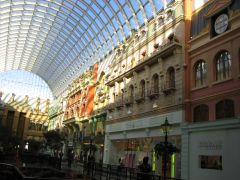
\includegraphics[width=.45\linewidth]{gfx/example_1}} \quad
        \subfloat[Pan ma signo.]
        {\label{fig:example-b}%
         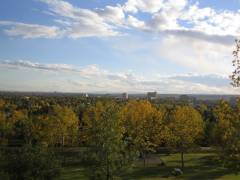
\includegraphics[width=.45\linewidth]{gfx/example_2}} \\
        \subfloat[Methodicamente o uno.]
        {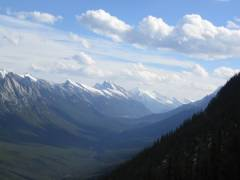
\includegraphics[width=.45\linewidth]{gfx/example_3}} \quad
        \subfloat[Titulo debitas.]
        {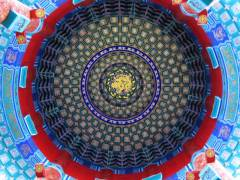
\includegraphics[width=.45\linewidth]{gfx/example_4}}
        \caption[Tu duo titulo debitas latente]{Tu duo titulo debitas
        latente.}\label{fig:example}
\end{figure}


%*****************************************
%*****************************************
%*****************************************
%*****************************************
%*****************************************

%\addtocontents{toc}{\protect\clearpage} % <--- just debug stuff, ignore
% %************************************************
\chapter{Math Test Chapter}\label{ch:mathtest} % $\mathbb{ZNR}$
%************************************************
Ei choro aeterno antiopam mea, labitur bonorum pri no. His no decore
nemore graecis. In eos meis nominavi, liber soluta vim cu. Sea commune
suavitate interpretaris eu, vix eu libris efficiantur.

\section{Some Formulas}
Due to the statistical nature of ionisation energy loss, large
fluctuations can occur in the amount of energy deposited by a particle
traversing an absorber element\footnote{Examples taken from Walter
Schmidt's great gallery: \\
\url{http://home.vrweb.de/~was/mathfonts.html}}.  Continuous processes
such as multiple
scattering and energy loss play a relevant role in the longitudinal
and lateral development of electromagnetic and hadronic
showers, and in the case of sampling calorimeters the
measured resolution can be significantly affected by such fluctuations
in their active layers.  The description of ionisation fluctuations is
characterised by the significance parameter $\kappa$, which is
proportional to the ratio of mean energy loss to the maximum allowed
energy transfer in a single collision with an atomic electron:
\graffito{You might get unexpected results using math in chapter or
section heads. Consider the \texttt{pdfspacing} option.}
\begin{equation}
\kappa =\frac{\xi}{E_{\textrm{max}}} %\mathbb{ZNR}
\end{equation}
$E_{\textrm{max}}$ is the maximum transferable energy in a single
collision with an atomic electron.
\[
E_{\textrm{max}} =\frac{2 m_{\textrm{e}} \beta^2\gamma^2 }{1 +
2\gamma m_{\textrm{e}}/m_{\textrm{x}} + \left ( m_{\textrm{e}}
/m_{\textrm{x}}\right)^2}\ ,
\]
where $\gamma = E/m_{\textrm{x}}$, $E$ is energy and
$m_{\textrm{x}}$ the mass of the incident particle,
$\beta^2 = 1 - 1/\gamma^2$ and $m_{\textrm{e}}$ is the electron mass.
$\xi$ comes from the Rutherford scattering cross section
and is defined as:
\begin{eqnarray*} \xi  = \frac{2\pi z^2 e^4 N_{\textrm{Av}} Z \rho
\delta x}{m_{\textrm{e}} \beta^2 c^2 A} =  153.4 \frac{z^2}{\beta^2}
\frac{Z}{A}
  \rho \delta x \quad\textrm{keV},
\end{eqnarray*}
where

\begin{tabular}{ll}
$z$          & charge of the incident particle \\
$N_{\textrm{Av}}$     & Avogadro's number \\
$Z$          & atomic number of the material \\
$A$          & atomic weight of the material \\
$\rho$       & density \\
$ \delta x$  & thickness of the material \\
\end{tabular}

$\kappa$ measures the contribution of the collisions with energy
transfer close to $E_{\textrm{max}}$.  For a given absorber, $\kappa$
tends
towards large values if $\delta x$ is large and/or if $\beta$ is
small.  Likewise, $\kappa$ tends towards zero if $\delta x $ is small
and/or if $\beta$ approaches $1$.

The value of $\kappa$ distinguishes two regimes which occur in the
description of ionisation fluctuations:

\begin{enumerate}
\item A large number of collisions involving the loss of all or most
  of the incident particle energy during the traversal of an absorber.

  As the total energy transfer is composed of a multitude of small
  energy losses, we can apply the central limit theorem and describe
  the fluctuations by a Gaussian distribution.  This case is
  applicable to non-relativistic particles and is described by the
  inequality $\kappa > 10 $ (\ie, when the mean energy loss in the
  absorber is greater than the maximum energy transfer in a single
  collision).

\item Particles traversing thin counters and incident electrons under
  any conditions.

  The relevant inequalities and distributions are $ 0.01 < \kappa < 10
  $,
  Vavilov distribution, and $\kappa < 0.01 $, Landau distribution.
\end{enumerate}


\section{Various Mathematical Examples}
If $n > 2$, the identity
\[
  t[u_1,\dots,u_n] = t\bigl[t[u_1,\dots,u_{n_1}], t[u_2,\dots,u_n]
  \bigr]
\]
defines $t[u_1,\dots,u_n]$ recursively, and it can be shown that the
alternative definition
\[
  t[u_1,\dots,u_n] = t\bigl[t[u_1,u_2],\dots,t[u_{n-1},u_n]\bigr]
\]
gives the same result.  

%*****************************************
%*****************************************
%*****************************************
%*****************************************
%*****************************************

%\include{multiToC} % <--- just debug stuff, ignore for your documents
% ********************************************************************
% Backmatter
%*******************************************************
\appendix
\cleardoublepage
\part{Appendix}
% %********************************************************************
% Appendix
%*******************************************************
% If problems with the headers: get headings in appendix etc. right
%\markboth{\spacedlowsmallcaps{Appendix}}{\spacedlowsmallcaps{Appendix}}
\chapter{Appendix Test}
Lorem ipsum at nusquam appellantur his, ut eos erant homero
concludaturque. Albucius appellantur deterruisset id eam, vivendum
partiendo dissentiet ei ius. Vis melius facilisis ea, sea id convenire
referrentur, takimata adolescens ex duo. Ei harum argumentum per. Eam
vidit exerci appetere ad, ut vel zzril intellegam interpretaris.

Errem omnium ea per, pro congue populo ornatus cu, ex qui dicant
nemore melius. No pri diam iriure euismod. Graecis eleifend
appellantur quo id. Id corpora inimicus nam, facer nonummy ne pro,
kasd repudiandae ei mei. Mea menandri mediocrem dissentiet cu, ex
nominati imperdiet nec, sea odio duis vocent ei. Tempor everti
appareat cu ius, ridens audiam an qui, aliquid admodum conceptam ne
qui. Vis ea melius nostrum, mel alienum euripidis eu.

\section{Appendix Section Test}
Ei choro aeterno antiopam mea, labitur bonorum pri no. His no decore
nemore graecis. In eos meis nominavi, liber soluta vim cu. Sea commune
suavitate interpretaris eu, vix eu libris efficiantur.

\graffito{More dummy text.}
Nulla fastidii ea ius, exerci suscipit instructior te nam, in ullum
postulant quo. Congue quaestio philosophia his at, sea odio autem
vulputate ex. Cu usu mucius iisque voluptua. Sit maiorum propriae at,
ea cum primis intellegat. Hinc cotidieque reprehendunt eu nec. Autem
timeam deleniti usu id, in nec nibh altera.

\section{Another Appendix Section Test}
Equidem detraxit cu nam, vix eu delenit periculis. Eos ut vero
constituto, no vidit propriae complectitur sea. Diceret nonummy in
has, no qui eligendi recteque consetetur. Mel eu dictas suscipiantur,
et sed placerat oporteat. At ipsum electram mei, ad aeque atomorum
mea.

\begin{table}
    \myfloatalign
  \begin{tabularx}{\textwidth}{Xll} \toprule
    \tableheadline{labitur bonorum pri no} & \tableheadline{que vista}
    & \tableheadline{human} \\ \midrule
    fastidii ea ius & germano &  demonstratea \\
    suscipit instructior & titulo & personas \\
    %postulant quo & westeuropee & sanctificatec \\
    \midrule
    quaestio philosophia & facto & demonstrated \\
    %autem vulputate ex & parola & romanic \\
    %usu mucius iisque & studio & sanctificatef \\
    \bottomrule
  \end{tabularx}
  \caption[Autem usu id]{Autem usu id.}
  \label{tab:moreexample}
\end{table}

Ei solet nemore consectetuer nam. Ad eam porro impetus, te choro omnes
evertitur mel. Molestie conclusionemque vel at, no qui omittam
expetenda efficiendi. Eu quo nobis offendit, verterem scriptorem ne
vix.

  
\begin{lstlisting}[float,caption=A floating example]
for i:=maxint to 0 do
begin
{ do nothing }
end;
\end{lstlisting}
%********************************************************************
% Other Stuff in the Back
%*******************************************************
\cleardoublepage%*******************************************************
% Glossary
%*******************************************************

\begingroup
\let\clearpage\relax
\let\cleardoublepage\relax
\let\cleardoublepage\relax

% to have the bib a bit from the rest in the toc
\chapter*{Glossary}
\addtocontents{toc}{\protect\vspace{\beforebibskip}}
\addcontentsline{toc}{chapter}{\tocEntry{Glossary}}

\printglossaries

\endgroup

\cleardoublepage%********************************************************************
% Bibliography
%*******************************************************
% work-around to have small caps also here in the headline
\manualmark
\markboth{\spacedlowsmallcaps{\bibname}}{\spacedlowsmallcaps{\bibname}} % work-around to have small caps also
%\phantomsection 
\refstepcounter{dummy}
% \addtocontents{toc}{\protect\vspace{\beforebibskip}} % to have the bib a bit from the rest in the toc
% \addcontentsline{toc}{chapter}{\tocEntry{\bibname}}
\bibliographystyle{plainnat}
\bibliography{../references.bib}

% \cleardoublepage\pagestyle{empty}

\hfill

\vfill


\pdfbookmark[0]{Colophon}{colophon}
\section*{Colophon}
This document was typeset using the typographical look-and-feel \texttt{classicthesis} developed by Andr\'e Miede. 
The style was inspired by Robert Bringhurst's seminal book on typography ``\emph{The Elements of Typographic Style}''. 
\texttt{classicthesis} is available for both \LaTeX\ and \mLyX: 
\begin{center}
\url{http://code.google.com/p/classicthesis/}
\end{center}
Happy users of \texttt{classicthesis} usually send a real postcard to the author, a collection of postcards received so far is featured here: 
\begin{center}
\url{http://postcards.miede.de/}
\end{center}
 
\bigskip

\noindent\finalVersionString

%Hermann Zapf's \emph{Palatino} and \emph{Euler} type faces (Type~1 PostScript fonts \emph{URW
%Palladio L} and \emph{FPL}) are used. The ``typewriter'' text is typeset in \emph{Bera Mono}, 
%originally developed by Bitstream, Inc. as ``Bitstream Vera''. (Type~1 PostScript fonts were made 
%available by Malte Rosenau and
%Ulrich Dirr.)

%\paragraph{note:} The custom size of the textblock was calculated
%using the directions given by Mr. Bringhurst (pages 26--29 and
%175/176). 10~pt Palatino needs  133.21~pt for the string
%``abcdefghijklmnopqrstuvwxyz''. This yields a good line length between
%24--26~pc (288--312~pt). Using a ``\emph{double square textblock}''
%with a 1:2 ratio this results in a textblock of 312:624~pt (which
%includes the headline in this design). A good alternative would be the
%``\emph{golden section textblock}'' with a ratio of 1:1.62, here
%312:505.44~pt. For comparison, \texttt{DIV9} of the \texttt{typearea}
%package results in a line length of 389~pt (32.4~pc), which is by far
%too long. However, this information will only be of interest for
%hardcore pseudo-typographers like me.%
%
%To make your own calculations, use the following commands and look up
%the corresponding lengths in the book:
%\begin{verbatim}
%    \settowidth{\abcd}{abcdefghijklmnopqrstuvwxyz}
%    \the\abcd\ % prints the value of the length
%\end{verbatim}
%Please see the file \texttt{classicthesis.sty} for some precalculated 
%values for Palatino and Minion.
%
%    \settowidth{\abcd}{abcdefghijklmnopqrstuvwxyz}
%    \the\abcd\ % prints the value of the length





% \cleardoublepage%*******************************************************
% Declaration
%*******************************************************
\refstepcounter{dummy}
\pdfbookmark[0]{Declaration}{declaration}
\chapter*{Declaration}
\thispagestyle{empty}
Put your declaration here.
\bigskip
 
\noindent\textit{\myLocation, \myTime}

\smallskip

\begin{flushright}
    \begin{tabular}{m{5cm}}
        \\ \hline
        \centering\myName \\
    \end{tabular}
\end{flushright}

% ********************************************************************
% Game Over: Restore, Restart, or Quit?
%*******************************************************
\end{document}
% ********************************************************************
